\documentclass{ximera}

%\addPrintStyle{..}

\begin{document}
	\author{Bart Lambregs}
	\xmtitle{Denkvragen}{}
    \xmsource\xmuitleg

\begin{exercise}
	Als de grootte van de snelheid van een voorwerp toeneemt, neemt de versnelling dan noodzakelijkerwijs ook toe? Motiveer je antwoord.
\end{exercise}

\begin{exercise}
	Kan de gemiddelde snelheid van een deeltje over een gegeven tijdsinterval gelijk zijn aan nul, terwijl de grootte van de snelheid over een kortere tijdsduur binnen dat tijdsinterval verschillend is van nul? Verklaar je antwoord.
\end{exercise}

\begin{exercise}
	Geef een voorbeeld waarin zowel de snelheids- als de versnellingscomponent negatief zijn.
\end{exercise}

\begin{exercise}
	Wanneer een voorwerp zich met een constante snelheid verplaatst, verschilt de gemiddelde snelheid over een willekeurig tijdsinterval dan van de ogenblikkelijke snelheid op een willekeurig moment?
\end{exercise}



\begin{exercise}
    Een puntmassa voert een eenparig veranderlijke rechtlijnige beweging uit over het tijdsinterval [\SI{0}{s},\SI{2}{s}] met beginsnelheid en beginpositie van respectievelijk \SI{0}{m/s} en \SI{0}{m}. De versnelling is \SI{3}{m/s^2}. Waarom kan je onmiddellijk stellen dat als in het tijdsinterval de tijd half om is, de puntmassa nog niet halfweg is?
        %\item Breng, zoals de opgelegde werkwijze bij het oplossen van vraagstukken vereist, zowel het gegeven als het gevraagde (hier het te bewijzen) in symbolen.
    \begin{question} Leg in woorden uit op welke manier je onmiddellijk kan inzien dat het te bewijzen juist is. \end{question}
    \begin{question} Controleer het te bewijzen via de numerieke waarden van dit vraagstuk.                      \end{question}
    \begin{question} Geef nu het bewijs.                                                                         \end{question}
\end{exercise}

% Vraagstukken die focussen op wiskundige aspecten

\begin{exercise}
	Een massa vertrekt vanuit rust om een eenparig versnelde rechtlijnige beweging uit te voeren. Als haar beginpositie \SI{0}{m} is, welke van de volgende betrekkingen is dan juist?
	\begin{multipleChoice}
		\choice{$t=\frac{x}{2v}$}
		\choice[correct]{$t=\frac{2x}{v}$}
		\choice{$t=\frac{v}{2x}$}
		\choice{$t=\frac{2v}{x}$}
	\end{multipleChoice}
\end{exercise}

\begin{exercise}
	De snelheid van een lichaam dat vanuit rust vrij valt, bedraagt na een valafstand $x$:
	\begin{multipleChoice}
		\choice{$v=2gx$}
		\choice[correct]{$v=\sqrt{2gx}$}
		\choice{$v=gx$}
		\choice{$v=\sqrt{\frac{gx}{2}}$}
	\end{multipleChoice}
	\begin{oplossing}
		$v=gt=g\sqrt{\frac{2x}{g}}=\sqrt{2gx}$
	\end{oplossing}
\end{exercise}

\begin{exercise}
	Laat zien dat voor een EVRB volgende formule geldt: 
	\begin{eqnarray*}
		v^2=v_0^2+2a\Delta x
		%v^2=v_0^2+2a(x-x_0)
	\end{eqnarray*}

	\begin{oplossing}
		Uit $v=v_0+at$ volgt:
		\begin{eqnarray*}
			v^2&=&v_0^2+2v_0at+a^2t^2\\
			&=&v_0^2+2a(v_0t+\frac{1}{2}at^2)\\
			&=&v_0^2+2ax
		\end{eqnarray*}
	\end{oplossing}
\end{exercise}


% Denkvragen over grafische voorstellingen

\begin{exercise}
	Teken de overeenkomstige $x(t)$- en $a(t)$-grafiek bij de gegeven $v(t)$-grafiek. Ga ervan uit dat $x_0=\SI{0}{m}$.

	\begin{image}
    \begin{tikzpicture}[xscale=0.5]
        \draw[->] (0,0) -- (32,0) node[right, font=\Large] {$t$};
        \draw[->] (0,0) -- (0,13) node[left, font=\Large] {$v$};
        
        % \draw[dashed] (0,12) -- (5,12);
        % \draw[dashed] (5,0) -- (5,12);
        \draw[dashed] (15,4) -- (15,0) node[below] {$t_1$};
        
        % \foreach \x in {0,5,15,30}
        %     \draw (\x,0) -- (\x,-0.2) node[below] {\x};
        % \foreach \y in {4,8,12}
        %     \draw (0,\y) -- (-0.2,\y) node[left] {\y};
        
        \draw[thick] (0,8) -- (15,4) -- (30,4);
		
		% Define and label the origin
  		\coordinate (O) at (0,0);
  		\node[left] at (O) {$O$};

  		% Draw a small filled circle at O
  		\node at (O) [circle, fill, inner sep=1.5pt]{};

    \end{tikzpicture}	
    \end{image}
    \captionof{figure}{Snelheidsverloop in functie van de tijd}

\end{exercise}

% Old one
% \begin{image}[0.3\textwidth]
% 	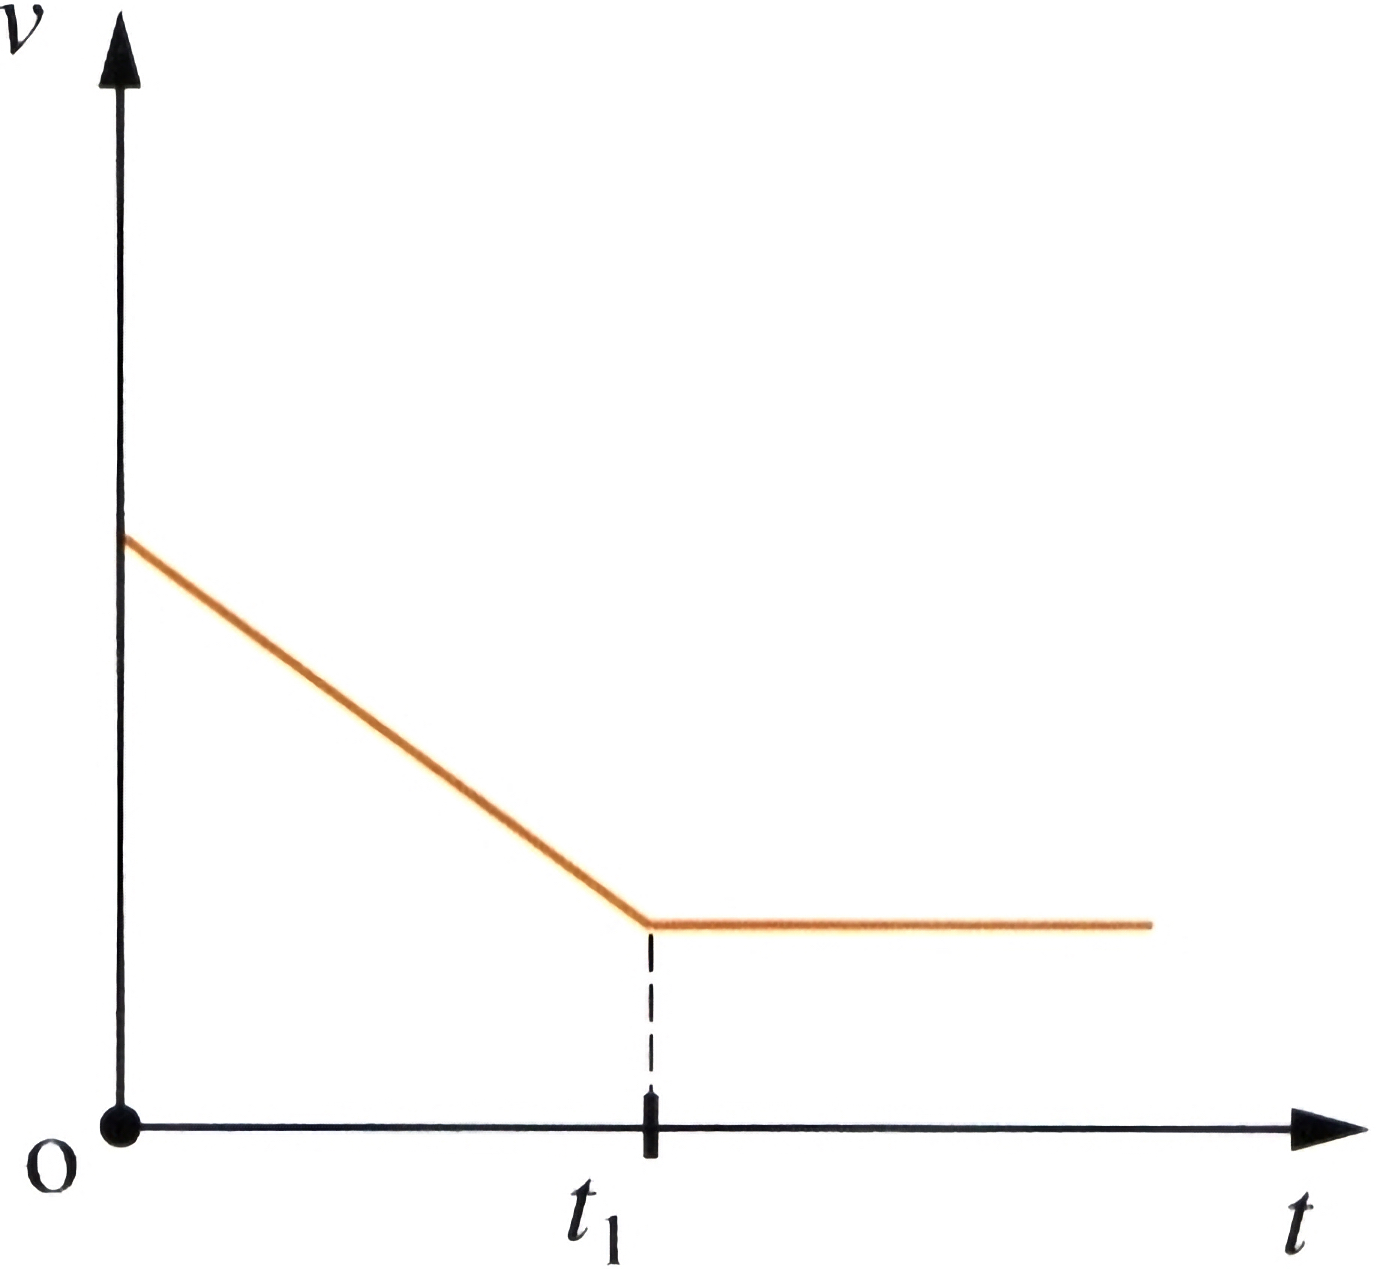
\includegraphics[width=\textwidth]{v(t)}
% \end{image}

\begin{exercise}
	De snelheid van een deeltje voldoet aan $v=at$ waarin $a$ constant en negatief is. De plaats van het deeltje wordt voorgesteld door $x$. Aangenomen wordt dat $x=0\rm\,m$ op het ogenblik $t=0\rm\,s$. 
	
	Welke grafiek geeft het juiste verloop van $x(t)$?

	\begin{multipleChoice}
		\choice{
			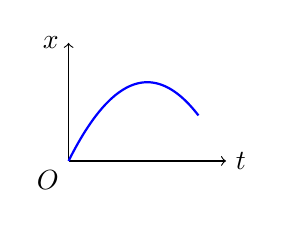
\begin{tikzpicture}[scale=0.5]
			  \draw[->] (0,0) -- (0,3) node[left]{$x$};
			  \draw[->] (0,0) -- (4,0) node[right]{$t$};
			  \node[below left] at (0,0) {$O$};
			  \draw[blue,thick, domain=0:3.3, samples=100] plot (\x,{2*\x -0.5*\x*\x});
			\end{tikzpicture}
		}
		\choice{
			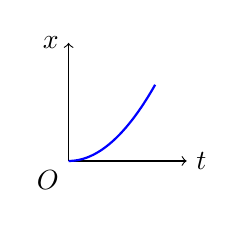
\begin{tikzpicture}[scale=0.5]
				\draw[->] (0,0) -- (0,3) node[left]{$x$};
				\draw[->] (0,0) -- (3,0) node[right]{$t$};
				\node[below left] at (0,0) {$O$};
				\draw[blue,thick, domain=0:2.2, samples=100] plot (\x,{0.4*\x*\x});
			\end{tikzpicture}
		}
		\choice[correct]{
			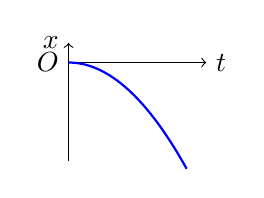
\begin{tikzpicture}[scale=0.5]
			  \draw[->] (0,0) -- (0,3) node[left]{$x$};
			  \draw[->] (0,2.5) -- (3.5,2.5) node[right]{$t$};
			  \node[left] at (0,2.5) {$O$};
			  \draw[blue,thick, domain=0:3, samples=100] plot (\x,{2.5 -0.3*\x*\x});
			\end{tikzpicture}
		}
		\choice{
			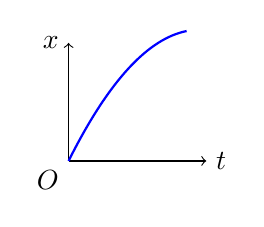
\begin{tikzpicture}[scale=0.5]
				\draw[->] (0,0) -- (0,3) node[left]{$x$};
				\draw[->] (0,0) -- (3.5,0) node[right]{$t$};
				\node[below left] at (0,0) {$O$};
				\draw[blue,thick, domain=0:3, samples=100] plot (\x,{2*\x -0.3*\x*\x});
			\end{tikzpicture}	
		}
	\end{multipleChoice}
\end{exercise}

\begin{exercise}
	Beargumenteer het gebruik van het model van een eenparig versnelde rechtlijnige beweging (EVRB) voor de vrije beweging van een wagentje op een helling. 
	Denk daarbij aan een proefneming die we in de klas deden. 
	De notie kracht moet je hier even buiten beschouwing laten.
	Beschrijf hierbij de beweging van het wagentje en de bijbehorende grafieken van \(x(t), v(v) \text{ en } a(t)\)
	\begin{oplossing}
		Het model beschrijft de meetgegevens accuraat.

		M.a.w. zijn de meetgegevens van de positie van het wagentje op de helling in functie van de tijd, gemeten met een (ultrasone) positiesensor, accuraat te beschrijven met de plaatsfunctie van een eenparig versnelde beweging.

		\emph{Toelichting}.
		De vraag gaat over de relatie tussen de theorie en de realiteit. Het is maar door metingen te doen dat we kunnen nagaan of gevolgen van de theorie (in dit geval bijvoorbeeld dat de positie kwadratisch in de tijd verloopt voor een beweging met constante versnelling) overeenkomen met de realiteit. In het gegeven geval van een wagentje op een helling, is bijvoorbeeld een model van constante snelheid niet van toepassing. Het zou immers impliceren dat het wagentje niet van zin kan veranderen. Dat laatste wordt door metingen of waarnemingen weerlegd.

		We spreken over een \textit{falsifieerbaar} model. Dat betekent dat zolang het niet weerlegd wordt, het geldig blijft. Je kan het alleen `vals' maken door een situatie te tonen waarin het \textit{niet} werkt.
	\end{oplossing} 
\end{exercise}

% Denkvragen over de valbeweging

\begin{exercise}
	Kan de bewegingszin van een voorwerp omkeren terwijl de versnelling gelijk blijft? Zo ja, geef dan een voorbeeld. Zo nee, leg uit waarom dat niet kan.
	\begin{oplossing}
		Ja, dat kan. Als je een bal opwerpt zal op het hoogste punt de bewegingszin omdraaien terwijl de versnelling gelijk blijft. We kunnen immers een verticale worp modelleren als een EVRB. Kiezen we de referentieas om de beweging te beschrijven omhoog, dan is de snelheid van de bal positief bij het naar boven bewegen en negatief wanneer hij naar beneden komt, terwijl de verandering van de snelheid in de tijd (de versnelling) systematisch gelijk is aan de negatieve valversnelling.
	\end{oplossing}
\end{exercise}
\todo{Eventueel uitleg aanpassen naar de situatie van een wagentje op een helling. Dan is deze vraag niet gekoppeld aan de context van een valbeweging, die later behandeld wordt.}

\begin{exercise}
	Kan een voorwerp dat een positieve versnelling heeft een negatieve snelheid hebben? Kan het omgekeerde ook?% Licht je antwoord toe.
	\begin{oplossing}
		Ja, dat kan. Neem bijvoorbeeld een voorwerp dat je verticaal omhoog gooit. Als je de referentieas waarmee je de beweging wil beschrijven verticaal naar benden kiest, zal de versnelling van de beweging positief zijn en de snelheid negatief. De snelheid is negatief omdat je tegengesteld aan de as beweegt en de versnelling is positief omdat de snelheid minder negatief wordt.

		Het omgekeerde kan ook, draai gewoon de referentieas om.
	\end{oplossing}
\end{exercise}

\begin{exercise}
	Een lichaam wordt verticaal omhoog geworpen. De referentieas is omhoog gericht. Welke van de volgende $v(t)$-diagrammen geeft dan het juiste verloop van de snelheid weer?

	\begin{multipleChoice}
		\choice{
			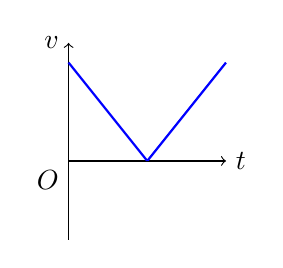
\begin{tikzpicture}[scale=0.5]
			  	\draw[->] (0,-2) -- (0,3) node[left]{$v$};
				\draw[->] (0,0) -- (4,0) node[right]{$t$};
				\node[below left] at (0,0) {$O$};
				\draw[blue,thick, domain=0:4, samples=100] plot (\x,{abs(-1.25*\x+2.5)});
			\end{tikzpicture}
		}
		\choice[correct]{
			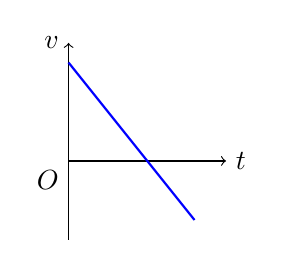
\begin{tikzpicture}[scale=0.5]
				\draw[->] (0,-2) -- (0,3) node[left]{$v$};
				\draw[->] (0,0) -- (4,0) node[right]{$t$};
				\node[below left] at (0,0) {$O$};
				\draw[blue,thick, domain=0:3.2, samples=100] plot (\x,{-1.25*\x+2.5});
			\end{tikzpicture}
		}
		\choice{
			\begin{tikzpicture}[scale=0.5]
				\draw[->] (0,-3) -- (0,2) node[left]{$v$};
				\draw[->] (0,0) -- (4,0) node[right]{$t$};
				\node[below left] at (0,0) {$O$};
				\draw[blue,thick, domain=0:3.2, samples=100] plot (\x,{1.25*\x-2.5});
			\end{tikzpicture}
		}
		\choice{
			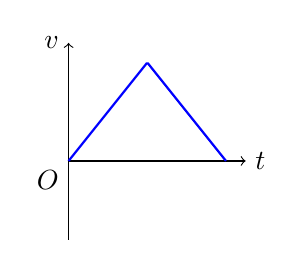
\begin{tikzpicture}[scale=0.5]
				\draw[->] (0,-2) -- (0,3) node[left]{$v$};
				\draw[->] (0,0) -- (4.5,0) node[right]{$t$};
				\node[below left] at (0,0) {$O$};
				\draw[blue,thick, domain=0:4, samples=100] plot (\x,{-abs(-1.25*\x+2.5)+2.5});
			\end{tikzpicture}	
		}
	\end{multipleChoice}

% Old one
% 	\begin{image}[.92\textwidth]
% 		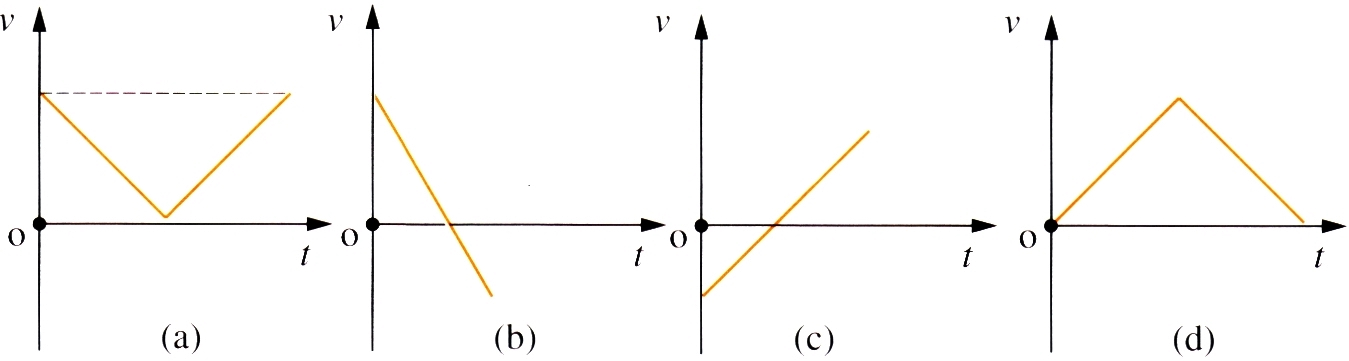
\includegraphics[width=\textwidth]{vw}
% 	\end{image}

	\begin{oplossing}
		Het juist antwoord is (b). De versnelling is constant waardoor de snelheid lineair moet verlopen in de tijd. Aangezien de referentieas naar boven is gekozen, moet de snelheid in het naar boven bewegen positief zijn. Dat is het geval bij (b).
	\end{oplossing}
\end{exercise}

\begin{exercise}
	Vanaf een klif laat men vanop dezelfde hoogte twee identieke bollen vallen. Men laat de tweede bol \'e\'en seconde later vallen dan de eerste. De luchtwrijving is \textit{niet} te verwaarlozen. Dan
	\begin{multipleChoice}
		\choice{zal de tweede bol iets later dan \'e\'en seconde na de eerste neerkomen.}
		\choice{zal de tweede bol iets vroeger dan \'e\'en seconde na de eerste neerkomen.}
		\choice[correct]{zal de tweede bol exact \'e\'en seconde na de eerste neerkomen.}
		\choice{kunnen we hieromtrent geen uitspraak doen bij gebrek aan gegevens.}
	\end{multipleChoice}
	\begin{oplossing}
		Voor beide bollen is de omstandigheid waarin ze vallen gelijk.
	\end{oplossing}
\end{exercise}

\begin{exercise}
	Vanop een grote hoogte laat men achtereenvolgens twee stenen vallen met een tussentijd van 2 seconden. 
	Op welke wijze verandert de afstand tussen beide stenen in de tijdsduur dat beide vallen?
	Geef een tijdsafhenkelijk voorschrift voor die afstand. 
	\begin{hint}
		Begin met een grafische voorstelling.
	\end{hint}
	\begin{oplossing}
		De afstand verandert lineair in functie van de tijd: $\Delta x(t)=gt_0\cdot t-\frac{1}{2}gt_0^2$ ($=\frac{1}{2}gt^2-\frac{1}{2}g(t-t_0)^2$ met $t\geq t_0=\SI{2}{s}$)
	\end{oplossing}
\end{exercise}

\begin{exercise}
	Aan de rand van een afgrond laat men een steen vallen. Op hetzelfde ogenblik werpt men een steen op. Zou het kunnen dat, als de afgrond diep genoeg is, beide stenen elkaar nog ontmoeten?

	\begin{oplossing}
		Aangezien de opgeworpen steen later (en zelfs hoger) begint met vallen en beide stenen eenzelfde versnelling hebben, kan op geen enkel moment de opgeworpen steen een grotere snelheid hebben dan de steen die wordt losgelaten. Dat laatste zou op het moment van inhalen nochtans op zijn minst het geval moeten zijn.

		In formules moet gelden, met $v_0$ een negatieve beginsnelheid:
		\begin{eqnarray*}
			\frac{1}{2}gt^2&=&v_0t+\frac{1}{2}gt^2.
		\end{eqnarray*}
		Dat is enkel het geval wanneer $t=0$.
	\end{oplossing}
\end{exercise}

\begin{exercise}
	Op de maan is de valversnelling slechts een zesde van die op de aarde. Als een voorwerp op de maan verticaal omhoog wordt gegooid, hoeveel maal hoger komt het dan dan een voorwerp dat met dezelfde beginsnelheid vanaf de aarde wordt opgeworpen?

	\begin{oplossing}
		De tijd die het voorwerp nodig heeft om tot zijn hoogste punt ($v=0$) te geraken, is $t=-\frac{v_0}{a}$ waarbij $a$ de negatieve versnelling op aarde of op de maan is. Met deze tijd en de gemiddelde snelheid gedurende de opwaartse beweging, kunnen we de bereikte hoogte uitdrukken in functie van de beginsnelheid $v_0$:
		\begin{eqnarray*}
			x=\bar{v}t=\frac{v_0+v}{2}\cdot\left(-\frac{v_0}{a}\right)=-\frac{v_0^2}{2a}
		\end{eqnarray*}
		Uit deze uitdrukking volgt dat de bereikte hoogte omgekeerd evenredig is met de versnelling. Op de maan zal het voorwerp dan ook zes keer zo hoog geraken.
	\end{oplossing}
\end{exercise}

\end{document}
